\chapter{Topologies for FPGA-to-FPGA communication}
\label{cha:topologies}

This chapter will describe in detail the topologies which can be setup to
connect the FPGAs using the QSFP ports to perform point-to-point communication
to each other. The first section of the chapter will introduce the possible
topologies which are feasible with the Noctua 32 FPGA system. The second
section will describe the prototypes which were developed to evaluate two
of the topologies to verify the functionality and compare the topologies
in terms of bandwidth capabilities specifically for the MIDG2 application.

\section{Topologies}

As the current available BSP for the Nallatech 520N boards only support serial
point-to-point communication between the FPGAs over direct connections, the
configurations to build a topology is limited by the number of ports which is 
4. The four ports would allow one FPGA to communicate simultaneously with 4
other FPGAs. To extend the communication beyond this, the FPGAs can either
communicate via MPI using the host processor or hop over the FPGAs via the
shortest path. Considering these criterion four topologies are feasible which
either use MPI or hops to extend the communication above the 4 nodes.


\subsection*{Terminologies}

To make the understanding of the topologies clear, this section would introduce
some terms which would be used to describe the topologies in the next sections.
The figure \ref{fig:simple_network} shows a network of two FPGAs.
The FPGAs act as the nodes in this network which are connected to each other
with a direct link. To not confuse with the cluster node which are connected to
each other using 100 Gb/s Intel Omni Path, the thesis will refer
these nodes as FPGA and cluster nodes as node in rest of the text. A network in
which all the nodes are connected to each other with direct FPGA-to-FPGA link
will be called an \textit{Isle}. The communication between isles is either done
using hops or MPI via host. The nodes within the isle can either be fully
connected or partially connected to each other.

\begin{figure}[h]%
    \centering
    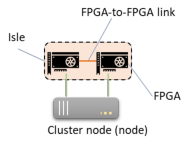
\includegraphics[width=0.4\textwidth]{images/simple_network}
    \caption{Simple network showing the network components}
    \label{fig:simple_network}
\end{figure}


\subsection{Within Node}
\label{sec:within_node}

The simplest topology possible is to connect the FPGAs of a node to each other
using a single channel or all the four channels forming an isle of two nodes as
shown in the figure \ref{fig:within_node}. The FPGAs can only communicate to
each other directly over the channel(s) utilizing the complete bandwidth of the
channels. The topologies can be scaled by adding more isles which communicate
to each other using MPI via the host using the Intel Omni Path. The topology
is simple and easy to setup. Applications which have large amount of data which
needs to be transferred between the processes can benefit from this topology by
efficiently partitioning and distributing the data among the isles and FPGAs.

\begin{figure}[h]%
    \centering
    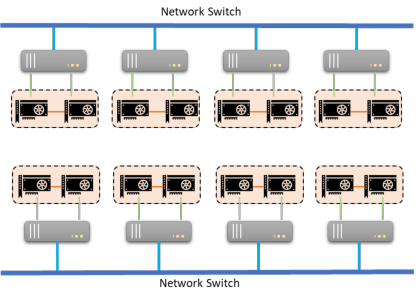
\includegraphics[width=0.7\textwidth]{images/within_node}
    \caption{Within Node topology with two node per isle}
    \label{fig:within_node}
\end{figure}

\subsection{Fully connected}
\label{sec:fully_connect}

The second topology extends the single node topology to two nodes such that
an isle contains four nodes fully connected to each other with separated 
point-to-point link as shown in figure \ref{fig:fully_connect}.
Each FPGA in this topology can communicate with three
other FPGAs simultaneously. Scaling the topology to more nodes can be achieved
in two ways. The first way is similar to within node where the isles communicate
using MPI. In this design, to decrease the overhead of exchanging data via the
MPI, the data should be collected on a single FPGA using the point-to-point
link and then exchanged via MPI. On the receiving end the process can be
reversed. Some more details of possible strategies to scale this design
effectively would be discussed in section \TODO{add reference} 

\begin{figure}[h]%
    \centering
    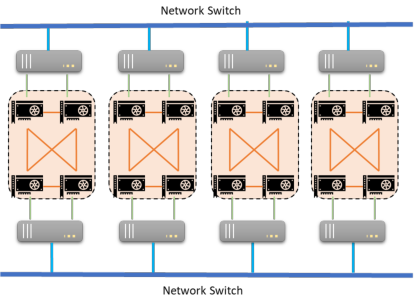
\includegraphics[width=0.7\textwidth]{images/full_connect}
    \caption{Fully connected topology of four FPGAs per isle}
    \label{fig:fully_connect}
\end{figure}

The second way to scale the design is to use the extra link left on the 
FPGAs to connect the isles to each other with two FPGA-to-FPGA links which is
described in the section \ref{sec:connected_graph}.

\subsection{Connected Graph}
\label{sec:connected_graph}

This topology is an extension of the fully connected topology of the fully
connected topology. The isle formed by the fully connected FPGAs is connected
to each other using the fourth free port forming a connected graph network
as show in figure \ref{fig:connected_graph}.
In this topology all the FPGAs can communicate to each other without requiring
any data communication via host. In addition to the knowledge of fully
connected mapping within the nodes, additional information about the neighboring
isles would be required to be stored or configured in the FPGAs at compile time
or at runtime. The additional information would be used by the FPGA to create
a mapping table to route packets to the destination FPGAs via the shortest path.
A data to be transferred from one FPGA to another in a different isle would
then have to hop over the FPGAs along the shortest path to reach
from source to destination.

\begin{figure}[h]%
    \centering
    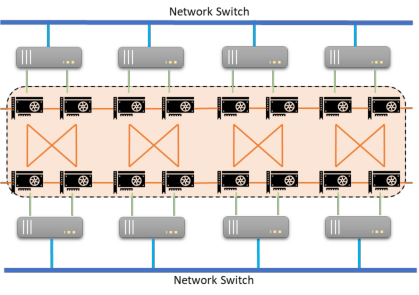
\includegraphics[width=0.7\textwidth]{images/connected_graph}
    \caption{Connected Graph with HOPs between fully connected groups}
    \label{fig:connected_graph}
\end{figure}

This thesis proposes this topology as possible scaling design and there was no
implementation and evaluation done for this topology as part of the thesis.

\subsection{Toroidal}
\label{sec:toroidal}

The last feasible topology for the FPGA network is the toroid. As explained by
\textcite{robertazzi_toroidal_1988}, A two dimensional toroidal network is
a network in which the nodes on the left and right boundaries and the
nodes on the top and bottom boundaries are connected to each other giving
a fully connected network. The length and breadth of the network can vary
depending upon the application requirements. As the maximum number of
connection for per node required in the toroidal network is 4, the toroidal
suits a lot to create a fully connected network of the FPGAs.

As Noctua has 32 FPGAs, two 4 X 4 torus as shown in figure \ref{fig:toroidal}
would be appropriate for connecting the FPGA giving an equidistant
hops in each direction. The actual routing and packet forwarding strategies
were not investigated in this thesis due to higher complexities
and lack of hardware resources to achieve a result as part of the thesis.

\begin{figure}[h]%
    \centering
    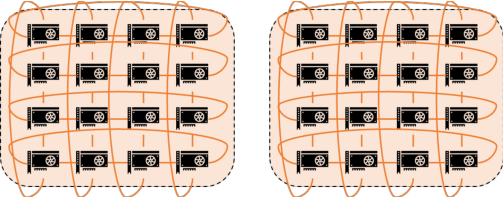
\includegraphics[width=0.7\textwidth]{images/torus}
    \caption{Two Toroidal network to connect 32 FPGAs}
    \label{fig:toroidal}
\end{figure}

\section{Prototypes to evaluate topologies}

This section would describe the prototypes developed to evaluate the topologies
introduced in sections \ref{sec:within_node} and \ref{sec:fully_connect}.

\subsection{Prototype for Within Node}

The implementation of the within node topology was simple and required very few
steps. To test the functionality and evaluate the achievable bandwidth with the
within node topology two OpenCL kernels \texttt{sender} and \texttt{collector}
were implemented. The code for the implemented kernels in shown in listing
\ref{code:within_node}. \texttt{sender} kernel uses the
\texttt{kernel\_output\_ch0} IO channel to send 256 bits of data per send.
The data and the length of data to be transferred in each kernel execution
is given by the host code through the parameters \texttt{input} and
\texttt{length} respectively. The host copies the data for \texttt{input}
buffer into the FPGA global memory using \texttt{enqueueWriteBuffer()} API.
The \texttt{collector} receives the data from the IO channel \texttt{kernel\_input\_ch0}
and writes into the global memory \texttt{output} which
is then read by the host using \texttt{enqueueReadBuffer()} to complete
the data exchange between the FPGAs.

\begin{CppCode} [caption=Kernels for within node prototype, frame=tlrb, label=code:within_node]
#pragma OPENCL EXTENSION cl_intel_channels : enable

channel float8 ch_eth_in __attribute((io("kernel_input_ch0")));
channel float8 ch_eth_out __attribute((io("kernel_output_ch0")));

__kernel void __attribute__ ((max_global_work_dim(0)))
sender(int length, __global float8 * restrict input)
{
    for(int i=0; i<length; ++i)
        write_channel_intel(ch_eth_out, input[i]);
}

__kernel void __attribute__ ((max_global_work_dim(0)))
collector(int length, __global float8 * restrict output)
{
    for(int i=0; i<length; ++i)
        output[i] = read_channel_intel(ch_eth_in);
}
\end{CppCode}

The same kernels are run on both FPGAs creating pairs of \texttt{sender}
and \texttt{collector} communicating over the channels as show in
figure \ref{fig:send_rcv} in the full duplex communication mode.

\begin{figure}[h]%
    \centering
    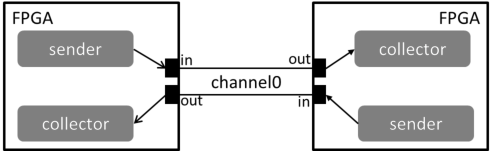
\includegraphics[width=0.7\textwidth]{images/send_recv}
    \caption{Communication structure of the kernels for within node topology with one channel}
    \label{fig:send_rcv}
\end{figure}

The host application was implemented using OpenCL C\+\+ classes to reduce the amount
of code and quickly test the functionality on the target platform. The host application
is responsible for reading the synthesized binary files (\texttt{.aocx}) and use the 
\texttt{cl::Program} class to reconfigure the FPGA with the new binaries. The host application
is also responsible to allocate the memories for the buffers \texttt{input} and
\texttt{output} in host memory and in device memory using \texttt{cl::Buffer} class.
The host code then sets all parameters for the kernels using the \texttt{cl::Kernel::setArg()}
method and queues the kernels for execution on the FPGA using \texttt{cl::CommandQueue::enqueueNDRangeKernel()}
method. The kernel used for prototype are implemented as a single work-item as it suits the 
serial IO channel communication.


\subsection*{Using all four channels for communication}

Another prototype was also developed for the within node topology which uses all the four channels
to communicate between the FPGAs. The benefit of this design is faster transfers for large data sizes
as communication is performed on all the channels parallely giving higher data rates. The modifications
done to the kernels to use all the four channels for communicating is shown in listing \ref{code:wn_fourch}

\begin{CppCode}[caption=Kernels for within node using four channels, frame=tlrb, label=code:wn_fourch]
#pragma OPENCL EXTENSION cl_intel_channels : enable
channel float8 ch_eth_in0 __attribute((io("kernel_input_ch0")));
channel float8 ch_eth_in1 __attribute((io("kernel_input_ch1")));
channel float8 ch_eth_in2 __attribute((io("kernel_input_ch2")));
channel float8 ch_eth_in3 __attribute((io("kernel_input_ch3")));

channel float8 ch_eth_out0 __attribute((io("kernel_output_ch0")));
channel float8 ch_eth_out1 __attribute((io("kernel_output_ch1")));
channel float8 ch_eth_out2 __attribute((io("kernel_output_ch2")));
channel float8 ch_eth_out3 __attribute((io("kernel_output_ch3")));

__kernel void __attribute__ ((max_global_work_dim(0)))
sender_all(int length, __global float8 * restrict input)
{
    for(int i=0; i<length; i=i+4)
    {
        write_channel_intel(ch_eth_out0, input[i]);
        write_channel_intel(ch_eth_out1, input[i+1]);
        write_channel_intel(ch_eth_out2, input[i+2]);
        write_channel_intel(ch_eth_out3, input[i+3]);
    }
}

__kernel void __attribute__ ((max_global_work_dim(0)))
collector_all(int length, __global float8 * restrict output)
{
    for(int i=0; i<length; i=i+4)
    {
        output[i] = read_channel_intel(ch_eth_in0);
        output[i+1] = read_channel_intel(ch_eth_in1);
        output[i+2] = read_channel_intel(ch_eth_in2);
        output[i+3] = read_channel_intel(ch_eth_in3);
    }
}
\end{CppCode}

\subsection{Prototype for Fully Connected}

The prototype for fully connected topology is an extension of the within node such that
it uses additional 2 channels for communicating with two other FPGAs. The prototype uses known
topology for communication which is derived from the fixed channel-FPGA pair formed by the
actual connections. The connection between the FPGAs are shown in figure \ref{fig:fc_topology}.

\begin{figure}[h]%
    \centering
    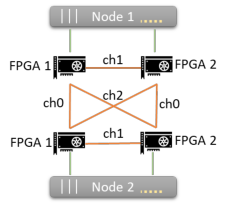
\includegraphics[width=0.4\textwidth]{images/fc_topology}
    \caption{Hardware setup for the fully connected topology}
    \label{fig:fc_topology}
\end{figure}

The FPGA implementation for fully connected topology also uses two OpenCL kernels
\texttt{sender\_all} and \texttt{collector\_all} for communication. The kernels
now use three channels which are shown in listing \ref{code:channels_fc}.
Each of the channel is used to communicate with 3 different FPGAs simultaneously.
For the prototypes, the host is designed to communicate same amount of data
to each FPGA although the kernels support sending and receiving different data
sizes from each channels. The host was limited to use same size to keep the prototype
simple in the starting. The integrated implementation requires using variable size and
a mechanism to identify and assign the sizes for each channel using partitioning
information is created which allows configuring the size dynamically.

\begin{CppCode} [caption=Channels used for fully connected topology, frame=tlrb, label=code:channels_fc]
#pragma OPENCL EXTENSION cl_intel_channels : enable
channel float8 ch_eth_in0 __attribute((io("kernel_input_ch0")));
channel float8 ch_eth_out0 __attribute((io("kernel_output_ch0")));

channel float8 ch_eth_in1 __attribute((io("kernel_input_ch1")));
channel float8 ch_eth_out1 __attribute((io("kernel_output_ch1")));

channel float8 ch_eth_in2 __attribute((io("kernel_input_ch2")));
channel float8 ch_eth_out2 __attribute((io("kernel_output_ch2")));
\end{CppCode}

The implementation of the \texttt{sender\_all} kernel is shown in listing \ref{code:send_fc}.
The kernel requires three separate memories and length, one for each of the channels, as
parameters from host. The kernels iterates over the input buffers for the maximum length
among the three lengths, sending 256 bits in each iterations over each channel. Individual
lengths for each channel is used to stop the sends for the specific channel in following
iterations. The structure shown in the listing creates three channel write units and three
memory load \ac{LSU} which allows sending the data parallely on all the three channels
in each iteration. 

\begin{CppCode} [caption=Sender Kernel for fully connected, frame=tlrb, label=code:send_fc]
__kernel void __attribute__ ((max_global_work_dim(0)))
sender_all(int length, int length1, int length2,
            __global float8 * restrict input,
            __global float8 * restrict input1,
            __global float8 * restrict input2)
{
    for(int i=0; i<length || i < length1 || i < length2; i++)
    {
        if (i < length)
            write_channel_intel(ch_eth_out0, input[i]);

        if (i < length1)
            write_channel_intel(ch_eth_out1, input1[i]);

        if (i < length2)
            write_channel_intel(ch_eth_out2, input2[i]);
    }
}
\end{CppCode}

The \texttt{collector\_all} used to receive data parallely from three FPGAs
was implemented similar to \texttt{sender\_all} kernel and requires same
number of parameters as shown in listing \ref{code:recv_fc}. The kernel
reads the data parallely from each of the channels and write them to the
corresponding buffers using the respective lengths for each channel
to limit the channel read.

\begin{CppCode} [caption=Collector Kernel for fully connected, frame=tlrb, label=code:recv_fc]
__kernel void __attribute__ ((max_global_work_dim(0)))
collector_all(int length, int length1, int length2,
            __global float8 * restrict output,
            __global float8 * restrict output1,
            __global float8 * restrict output2)
{
    for(int i=0; i<length || i < length1 || i < length2; i++)
    {
        if (i < length)
            output[i] = read_channel_intel(ch_eth_in0);

        if (i < length1)
            output1[i] = read_channel_intel(ch_eth_in1);
 
        if (i < length2)
            output2[i] = read_channel_intel(ch_eth_in2);
    }
}
\end{CppCode}

All four FPGAs use the same kernels to communicate to each other over the channels.
The structure of the communication is show in figure \ref{fig:fc_struc}

\begin{figure}[h]%
    \centering
    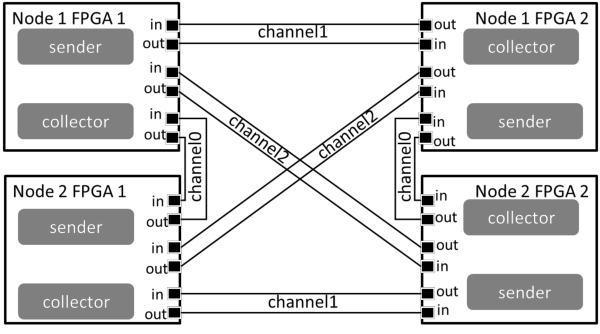
\includegraphics[width=0.7\textwidth]{images/fc_struc}
    \caption{Communication structure for the Fully connected kernels on each FPGA}
    \label{fig:fc_struc}
\end{figure}

The implementation of the host application for the fully connected design additionally
uses MPI. MPI is used to run the same host application on the 2 nodes. One each node
the host application programs both of the FPGAs with the same kernel binary and initializes
the kernel \texttt{sender\_all} and \texttt{collector\_all} on both FPGAs. Once the initialization
is done, the host starts the kernel using the \texttt{cl::CommandQueue::enqueueNDRangeKernel()}
method. The host waits for the completion of collector kernels on each FPGA, and then reads
the received data for verification. Additionally \texttt{MPI\_Barrier(MPI\_COMM\_WORLD)} functions
is used the synchronize the hosts. This synchronization helps to reduce the stalls
on the external channels.



